\documentclass[11pt,a4paper]{article}
\usepackage[margin=24mm]{geometry}
\usepackage[utf8]{inputenc}
\usepackage{tikz}
\usetikzlibrary{positioning}
\title{Scope filter for template iteration (subsystem views)}
\date{Created 2026-10-07 00:18 CEST}
\begin{document}
\maketitle
\paragraph{Scope and estimate.} Diagram templates iterate whole query results, so one view
of a large model is too wide. Add a scope clause to \texttt{\{\{\#each\}\}} that keeps only the
matches reachable from a root along named edge results, so one template renders one view per
subsystem (root as a config value). User decision 2026-10-07: engine extension \emph{and}
subsystem tags in the model, with a check that the two agree. ETA 90--120 minutes. No benchmark.
\paragraph{Syntax.}
\texttt{\{\{\#each L [within|touching|outside S from R] [except X]\}\}}.
\texttt{S}: comma-separated edge query labels, or the keyword \texttt{specializations}.
\texttt{R}: comma-separated declaration names. In \texttt{S} and \texttt{R} an item
\texttt{config:key} expands to the comma-separated config value, so one template renders every
view (amended during implementation: several roots, configurable sources). \texttt{X}: a query label.
\paragraph{Semantics.} The scope is the least set containing every declaration named
\texttt{R} and closed under: for each match of an edge label in \texttt{S} with a $+$ binding
inside the scope, add its $-$ binding targets ($\sim$ is never followed); with
\texttt{specializations}, add every declaration whose direct base is inside. A declaration is
\emph{inside} when it or an ancestor is in the set (ports go with their block). A node match
qualifies for \texttt{within} when inside; an edge match when every $\pm$ binding is inside;
\texttt{touching}: some $\pm$ binding is inside (node: inside); \texttt{outside}: not
\texttt{within}. \texttt{except X} drops matches whose declaration is a match of \texttt{X}.
Unknown labels and unresolved roots give an empty scope; a malformed clause is a template
parse error.
\paragraph{Ownership.} Query owns template semantics: \texttt{rewrite/template.rs} (parse and
dispatch) and a new crate-private \texttt{rewrite/scope.rs} (closure, membership). No public
symbol is added; \texttt{SYMBOLS.md} unchanged. Core read only (\texttt{Ir::parent},
\texttt{bases::bases}). View templates and the tag check live with the consumer model
(\texttt{02\_design/sze/halfarm/model/diagrams/}); upstreaming them as registered transforms
is a separate decision.
\paragraph{Tests.} Unit, in-memory model: \texttt{within} over composition (with ports via
ancestors), \texttt{touching} vs \texttt{within} on a connector, \texttt{outside} as complement,
\texttt{except}, \texttt{specializations}, multiple sources, \texttt{config:} root.
Counter-tests: a $\sim$ binding is not followed; an unknown source label and an unresolved
root render nothing; without the clause every match is emitted (the filter, not the query,
removes them); a malformed clause is rejected. Consumer check: tags versus scope report empty;
removing one tag and adding one wrong tag each produce exactly the expected line.
\paragraph{Budget and risks.} Closure is $O(\mathrm{iterations}\times\mathrm{edge\ matches})$,
computed once per \texttt{\#each} evaluation; specialization closure scans the declaration
table per iteration. Literal roots are matched by name; a duplicated name yields all
same-named declarations as roots (documented).
\paragraph{State and rollback.} Checkout on \texttt{feat/material-lobes} with the uncommitted
2026-10-06 structural-template change and another worker's uncommitted files (not touched).
No git writes from the Linux sandbox; the user branches and commits on Windows. Verification
in the sandbox build copy. Rollback: delete \texttt{scope.rs}, revert the \texttt{template.rs} hunks.
\begin{center}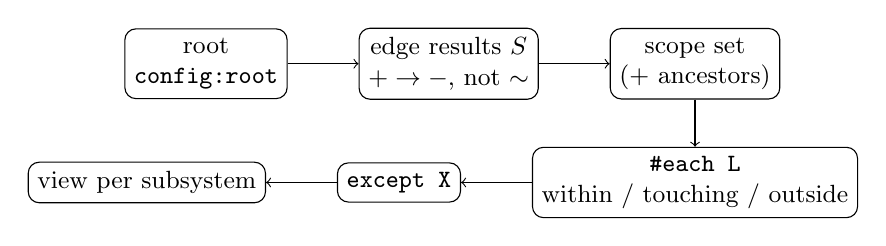
\begin{tikzpicture}[node distance=6mm and 9mm, every node/.style={draw, rounded corners, font=\small, align=center}]
\node (r) {root\\\texttt{config:root}};
\node (e) [right=of r] {edge results $S$\\$+ \rightarrow -$, not $\sim$};
\node (c) [right=of e] {scope set\\(+ ancestors)};
\node (f) [below=of c] {\texttt{\#each L}\\within / touching / outside};
\node (x) [left=of f] {\texttt{except X}};
\node (o) [left=of x] {view per subsystem};
\draw[->] (r) -- (e); \draw[->] (e) -- (c); \draw[->] (c) -- (f); \draw[->] (f) -- (x); \draw[->] (x) -- (o);
\end{tikzpicture}
\end{center}
\end{document}
